\documentclass{article}
\usepackage{amsmath}
\usepackage{amsthm}
\usepackage{amsfonts}
\usepackage{amssymb}
\usepackage{bbold}
\usepackage{dsfont}
\usepackage{graphicx}
\usepackage{cleveref}
\usepackage{bm}
\usepackage{booktabs}
\usepackage{siunitx}
\usepackage{xcolor}
\usepackage[utf8]{inputenc}
\usepackage[english]{babel}
\newtheorem{definition}{Definition}
\newtheorem{example}{Example}
\newcommand{\exP}[1]{\mathrm{e}^{#1}}
\newcommand{\dif}{\mathrm{d}}
\renewcommand{\vec}[1]{\mathbf{#1}}
\newcommand{\pdagger}{{\phantom{\dagger}}}
\newcommand{\state}[1]{\vert #1\rangle}
\newcommand{\cstate}[1]{\langle #1\vert}
\newcommand{\tr}[1]{\mathrm{tr}\left\{#1\right\}}
\newcommand{\trs}[2]{\, \mathrm{tr}_{#1}\{#2\}}
\newcommand{\expc}[3]{\langle #1\vert #2 \vert #3\rangle}
\usepackage[doi=false,url=false,isbn=false,backend=bibtex,style=nature,natbib=true,sorting=none]{biblatex}
\bibliography{bib.bib}
\usepackage{geometry}
\geometry{
	a4paper,
	total={170mm,257mm},
	left=20mm,
	top=20mm,
}
\begin{document}
	
\title{Fransson's model: Tests of implementation}
\author{Rudolf Smorka}
\maketitle
\section{Model}
The model considered for a chiral, single-stranded molecule, as proposed in Refs.~\cite{fransson2019chirality,fransson2020vibrational,Fransson_2021,fransson2021charge}, reads
\begin{align}
	\hat{H} &= \hat{H}_\mathrm{mol} + \hat{H}_\mathrm{env} + \hat{H}_\mathrm{sys-env}.
\end{align} 
The molecular Hamiltonian is modeled by a combination of the  Peierls and the Kane-Mele models. It consists of an electronic on-site, nearest-neighbor hopping, and next-to-nearest neighbor spin-orbit coupling (SOC), a Peierls electron-phonon coupling and vibrational contribution to SOC, and the harmonic phonon potential energy 
\begin{align}
	\hat{H}_\mathrm{mol} &= \hat{H}_\mathrm{el} + \hat{H}_\mathrm{el-ph} + \hat{H}_\mathrm{ph},\\
	\begin{split}
		\hat{H}_\mathrm{el} &= \sum_{j,\sigma} \varepsilon_{j\sigma}^\pdagger \hat{d}_{j\sigma}^\dagger \hat{d}_{j\sigma}^\pdagger - t_0 \sum_{j\sigma} (\hat{d}_{j\sigma}^\dagger \hat{d}_{j+1,\sigma}^\pdagger + \mathrm{h.c.}) +\\& \lambda_0^\pdagger\sum_{j\sigma\sigma'} (i\hat{d}_{j\sigma}^\dagger (\vec{v}_j^{(+)}\cdot \bm{\sigma})_{\sigma\sigma'}^\pdagger \hat{d}_{j+2,\sigma'}^\pdagger + \mathrm{h.c.}),
	\end{split}\\
	\hat{H}_\mathrm{el-ph} &= - t_1^\pdagger \sum_{j,\sigma}  \hat{d}_{j\sigma}^\dagger \hat{d}_{j+1\sigma}^\pdagger (\hat{a}_{j}^\dagger + \hat{a}_{j}^\pdagger) \\ & + \lambda_1^\pdagger\sum_{j\sigma} (i \hat{d}_{j\sigma}^\dagger (\vec{v}_j^{(+)} \cdot \bm{\sigma})_{\sigma\sigma'}^\pdagger \hat{d}_{j+2\sigma'}^\pdagger +\mathrm{h.c.})(\hat{a}_{j}^\dagger + \hat{a}_{j}^\pdagger),\label{eq:HelPh}\\
	\hat{H}_\mathrm{ph} &= \sum_{j} \omega_{j}^\pdagger \hat{a}_{j}^\dagger \hat{a}_{j}^\pdagger.
	 \label{eq:Hamiltonian_el_Fransson} 
\end{align}
This molecule is coupled to an environment of spin-full, noninteracting electrons
\begin{equation}
	H_\mathrm{env} = \sum_{\ell k\sigma} \varepsilon_{\ell k\sigma}^\pdagger c_{\ell k\sigma}^\dagger c_{\ell k\sigma}^\pdagger \label{eq:LeadHamiltonian}
\end{equation}
and the system-environment coupling is linear in the molecular and environmental operators (only at the first and last site of the molecule)
\begin{align}
	H_\mathrm{sys-env} &= \sum_{\sigma\sigma'}(\nu_{L\sigma\sigma'}^\pdagger c_{N_L\sigma}^\dagger d_{1\sigma'}^\pdagger + \nu_{R\sigma\sigma'}^\pdagger c_{1_R\sigma}^\dagger d_{\mathbb{M}\sigma'}^\pdagger + \mathrm{h.c.}). \label{eq:LeadSysHamiltonian}
\end{align} 
\section{Methods}
In the following, we compare the dynamics in the model defined above using a variety of methods. 
\begin{itemize}
	\item Exact diagonalization (ED): Valid for isolated molecule, phonons treated quantum-mechanically.
	\item Time-dependent variational principle based on a matrix-product state Ansatz (TDVP): Valid for isolated molecule, phonons treated quantum-mechanically.
	\item Hierarchical equations of motion in matrix product state representation (TT-HEOM): Valid for both isolated molecule and molecule coupled to leads, phonons treated quantum-mechanically.
	\item Hierarchical equations of motion in combination with Ehrenfest dynamics (MF-HEOM): Valid for purely electronic dynamics in both isolated molecule and molecule coupled to leads. Phonons approximated to be classical.
\end{itemize}
\newpage
\section{Comparison of dynamics within the TT-HEOM}
\subsection{Isolated: Hopping and Peierls distortion}
As in the previous report, the parameters are $L=3$, $t_0 = 1$, $t_1 = 0.1t_0$, $\omega_0 = 0.01t_0$.  GSE-TDVP data is not converged with respect to number of vibrational modes.
\begin{figure}[!h]
	\centering
	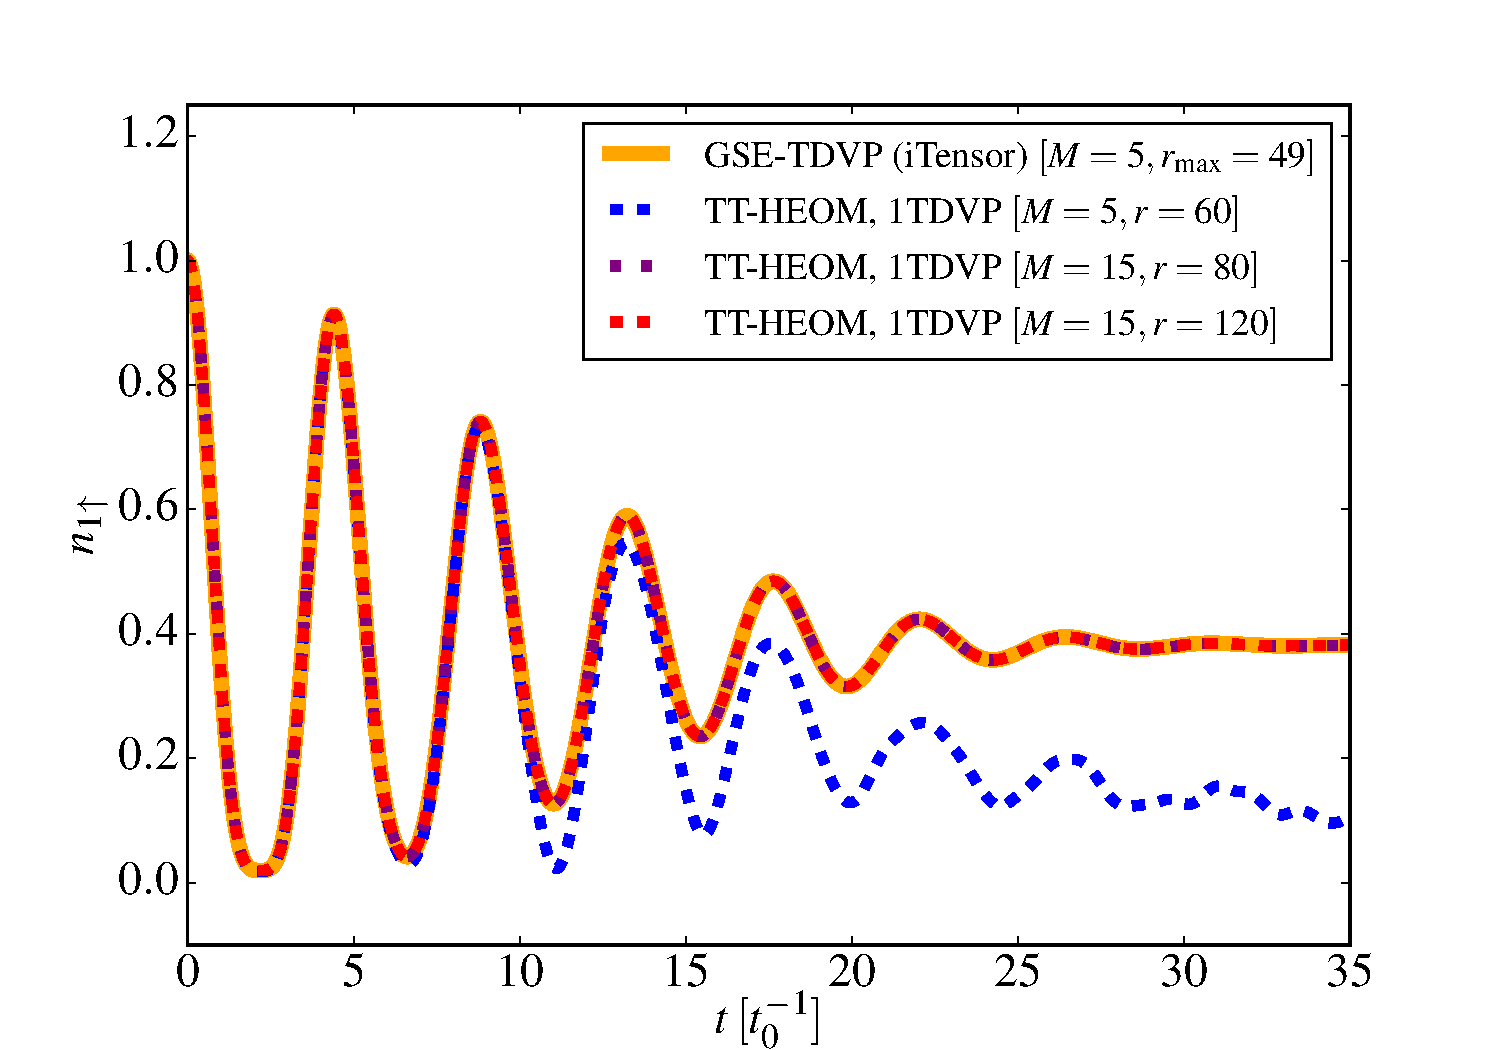
\includegraphics[width=0.8\textwidth]{figs/Comparison_TTHEOM_TDVP_ED_hop+onsite+tph_v2.pdf}
\end{figure}
The issue was in a factor $1/\sqrt{2}$ in the definition of the vibrational creation and annihilation operators in the code, which was overseen. 
\subsection{Coupled: Hopping and Onsite}
Parameters: $L=3$, $t_0 = 1.0$, $T=\SI{0.1}{\electronvolt}\approx \SI{1160}{\kelvin}$, $\Gamma = \vert \nu\vert^2 = t_0/4$, $V=t_0$.
\begin{figure}[!h]
	\centering
	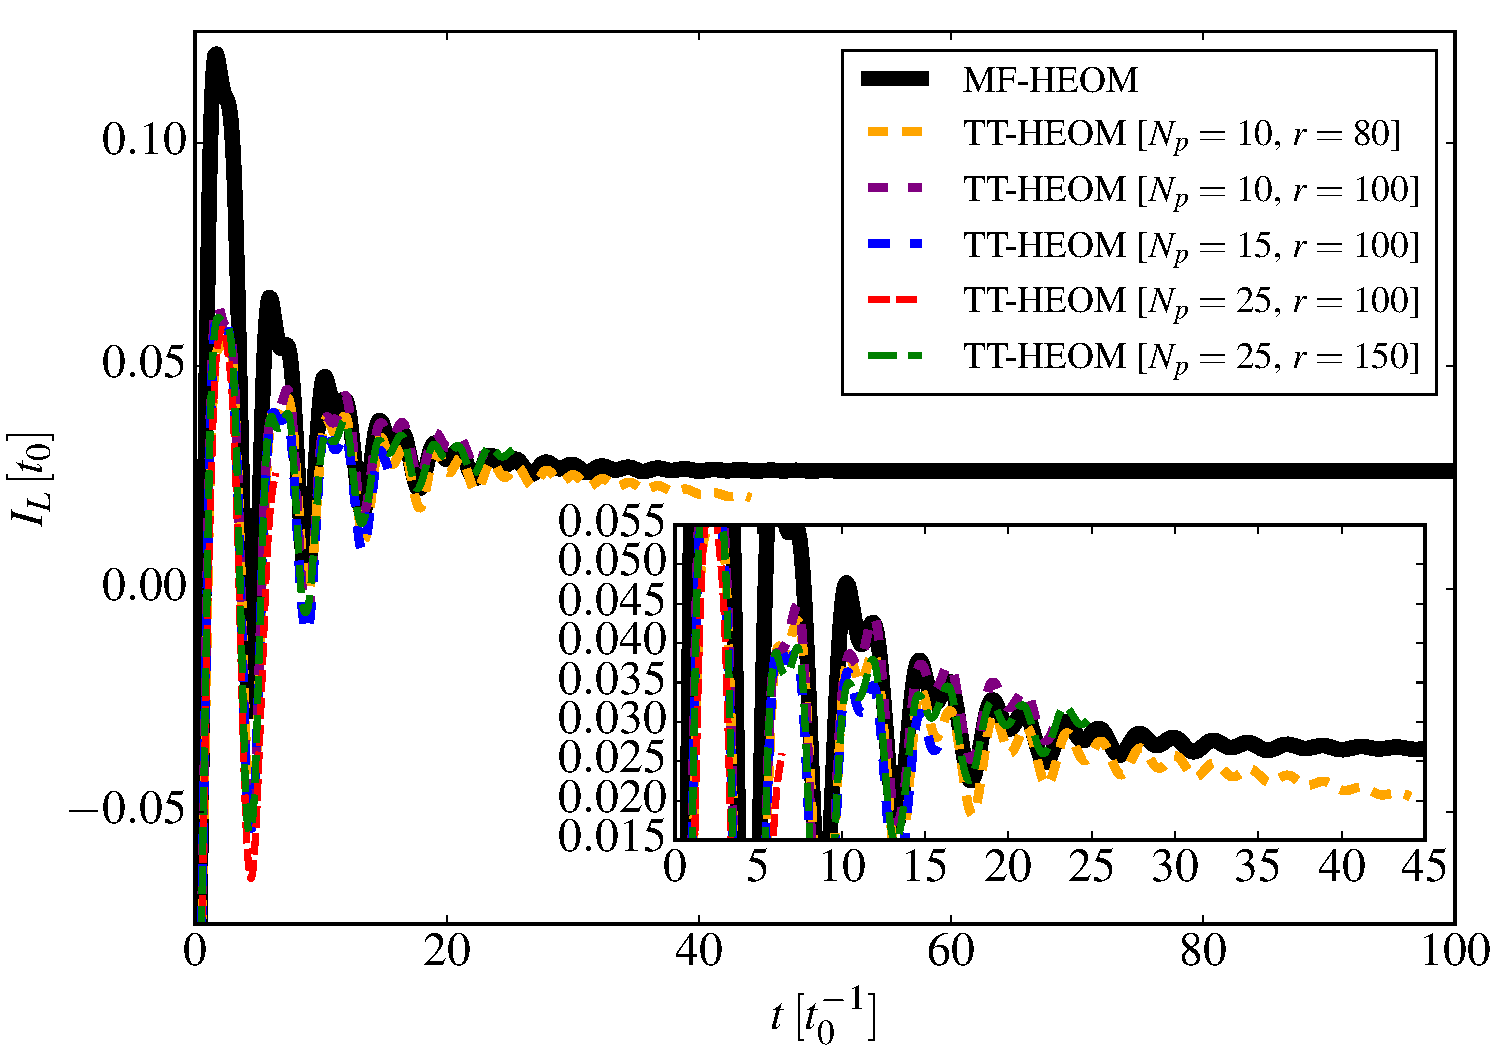
\includegraphics[width=0.8\textwidth]{figs/Comparison_TTHEOM_TDVP_ED_hop+onsite+SOC_V10.pdf}
\end{figure}

\section{Properties of the non-vibrating molecule}
Parameters: $t_0 = 1, \varepsilon_\uparrow = \varepsilon_\downarrow = -6t_0, \lambda_0 = t_0/40, \Gamma_0 = t_0/4, \beta = t_0/40$. 
\subsection{Current-voltage characteristics}
Due to absence of electronic interactions, the steady-state current can be obtained within the Landauer-Büttiker formalism.
The left lead is assumed to be ferromagnetic with polarization $P=0.5,-0.5$. This is modeled by a spin-dependent level-width function $\Gamma = \Gamma_0 (1+P\sigma^z)$ in Franssons work. However, a ferromagnetic metal also has a spin-gap between majority and minority spins $\mu_\mathrm{maj}-\mu_\mathrm{min} = \Delta_s$ (Stoner model), the influence of which we investigate separately.
\begin{figure}[!h]
	\centering
	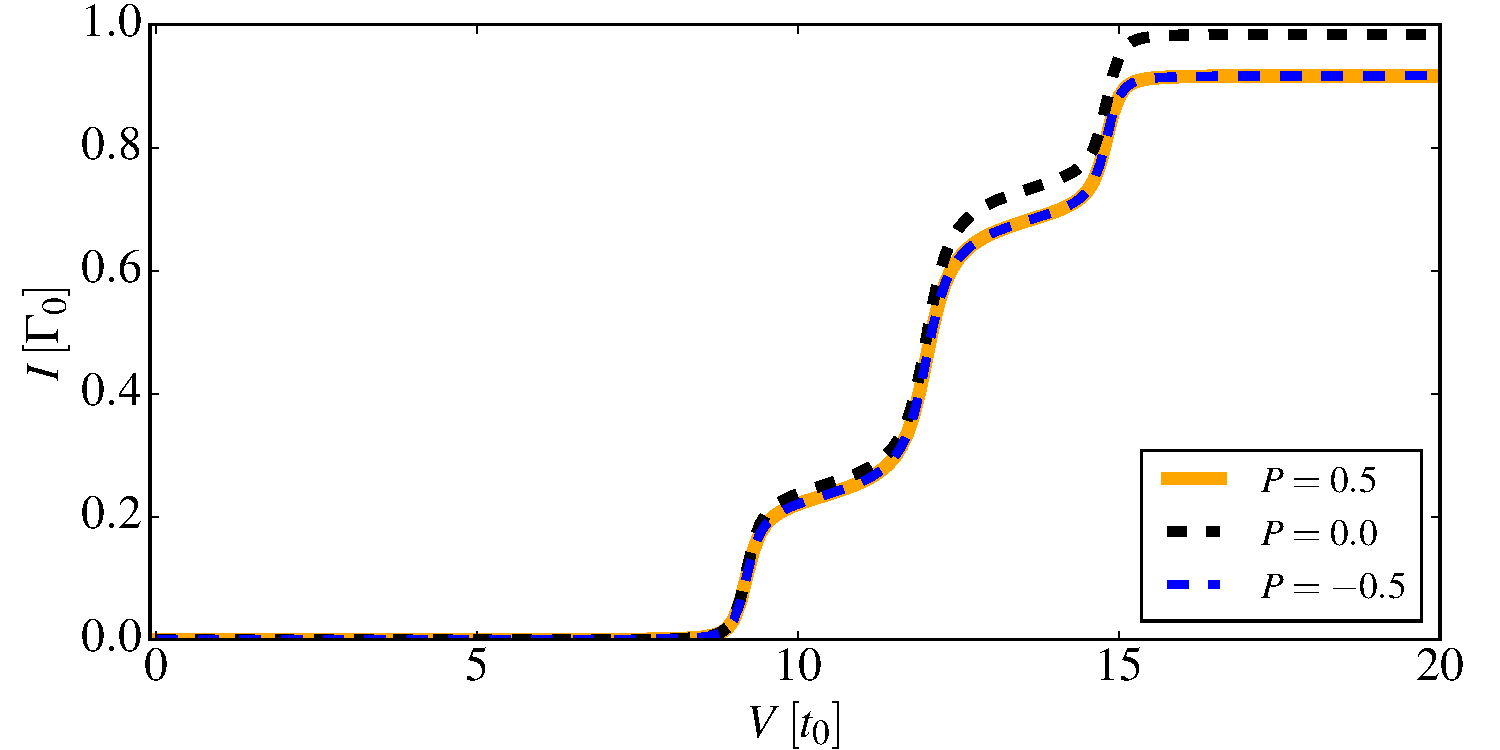
\includegraphics[width=0.6\textwidth]{figs/LB_1x3.pdf}
	\caption{$\mathbb{M}=1\times 3$}
\end{figure}
\begin{figure}[!h]
	\centering
	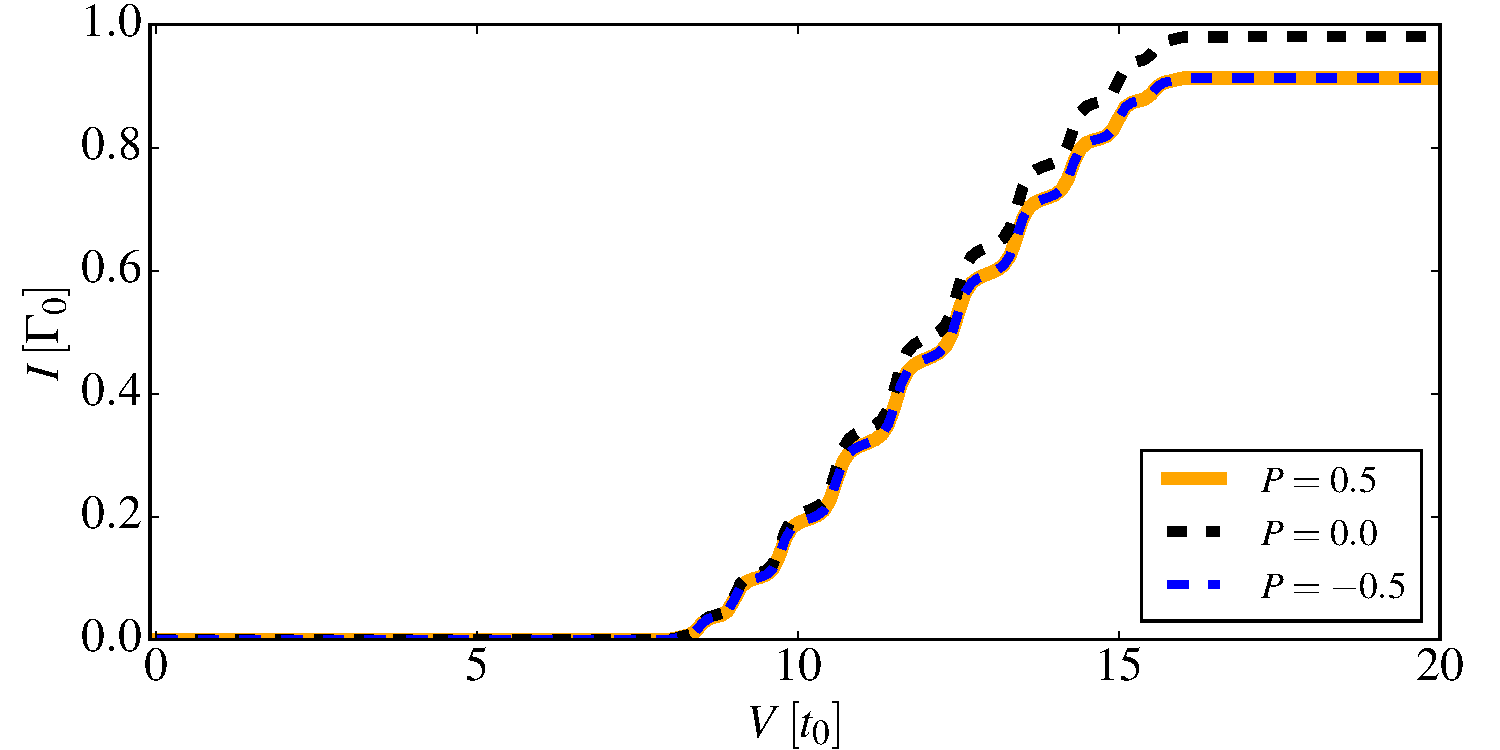
\includegraphics[width=0.6\textwidth]{figs/LB_4x3.pdf}
	\caption{$\mathbb{M}=4\times 3$}
\end{figure}
\begin{figure}[!h]
	\centering
	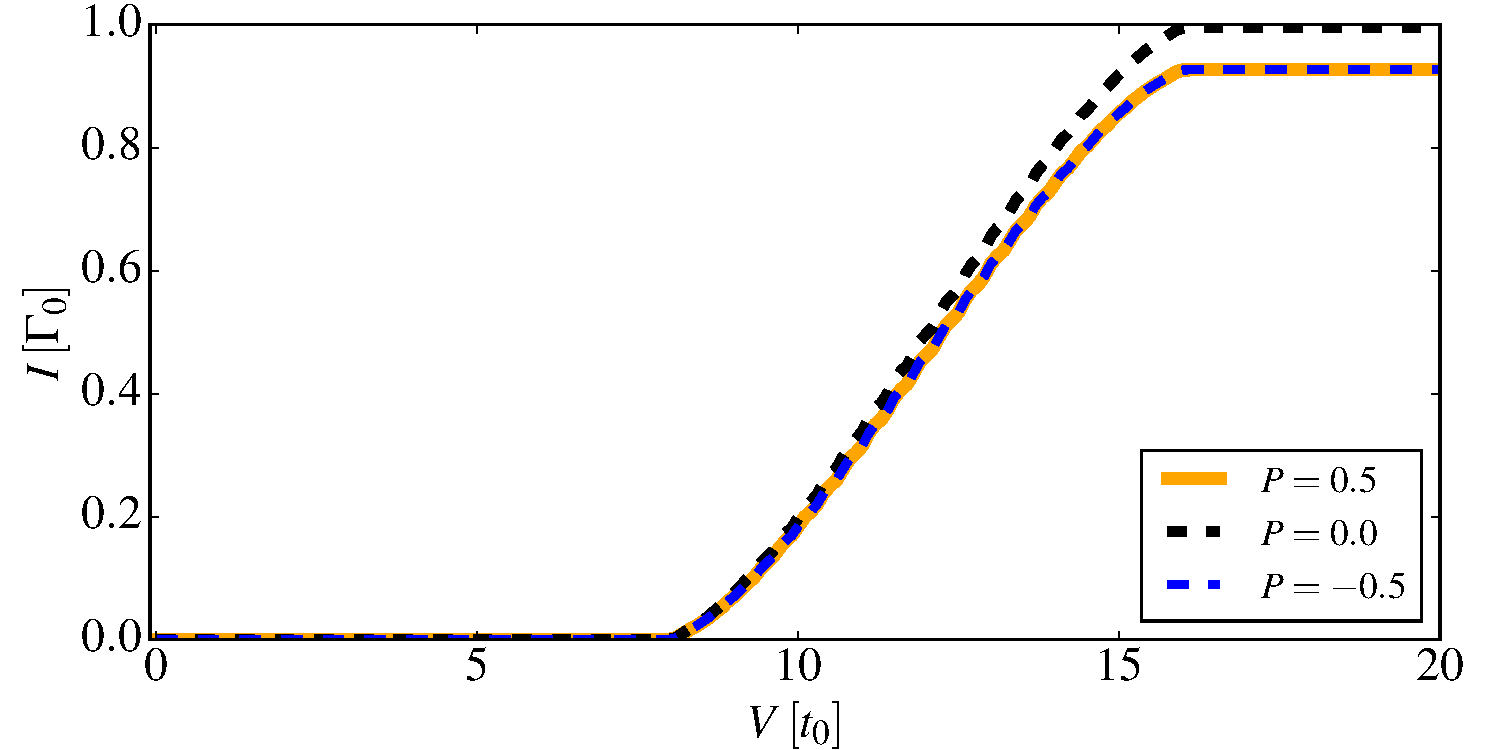
\includegraphics[width=0.6\textwidth]{figs/LB_8x4.pdf}
	\caption{$\mathbb{M}=8\times 4$}
\end{figure}
\subsection{Stationary electronic lattice occupation}
From the steady-state reduced density matrix obtained within the MF-HEOM, one can obtain local observables, as the electron population and local spin polarization.  
For $\mu_R>-4.5$ (or equivalently $V<8$), the electron population is nearly one. This is because due to the very large on-site energy $\varepsilon_m$, the full electronic spectrum is shifted to 
The electron population at each site changes discontinuously for each $\mu_R \approx \varepsilon_n$. 
\begin{figure}[!h]
	\centering
	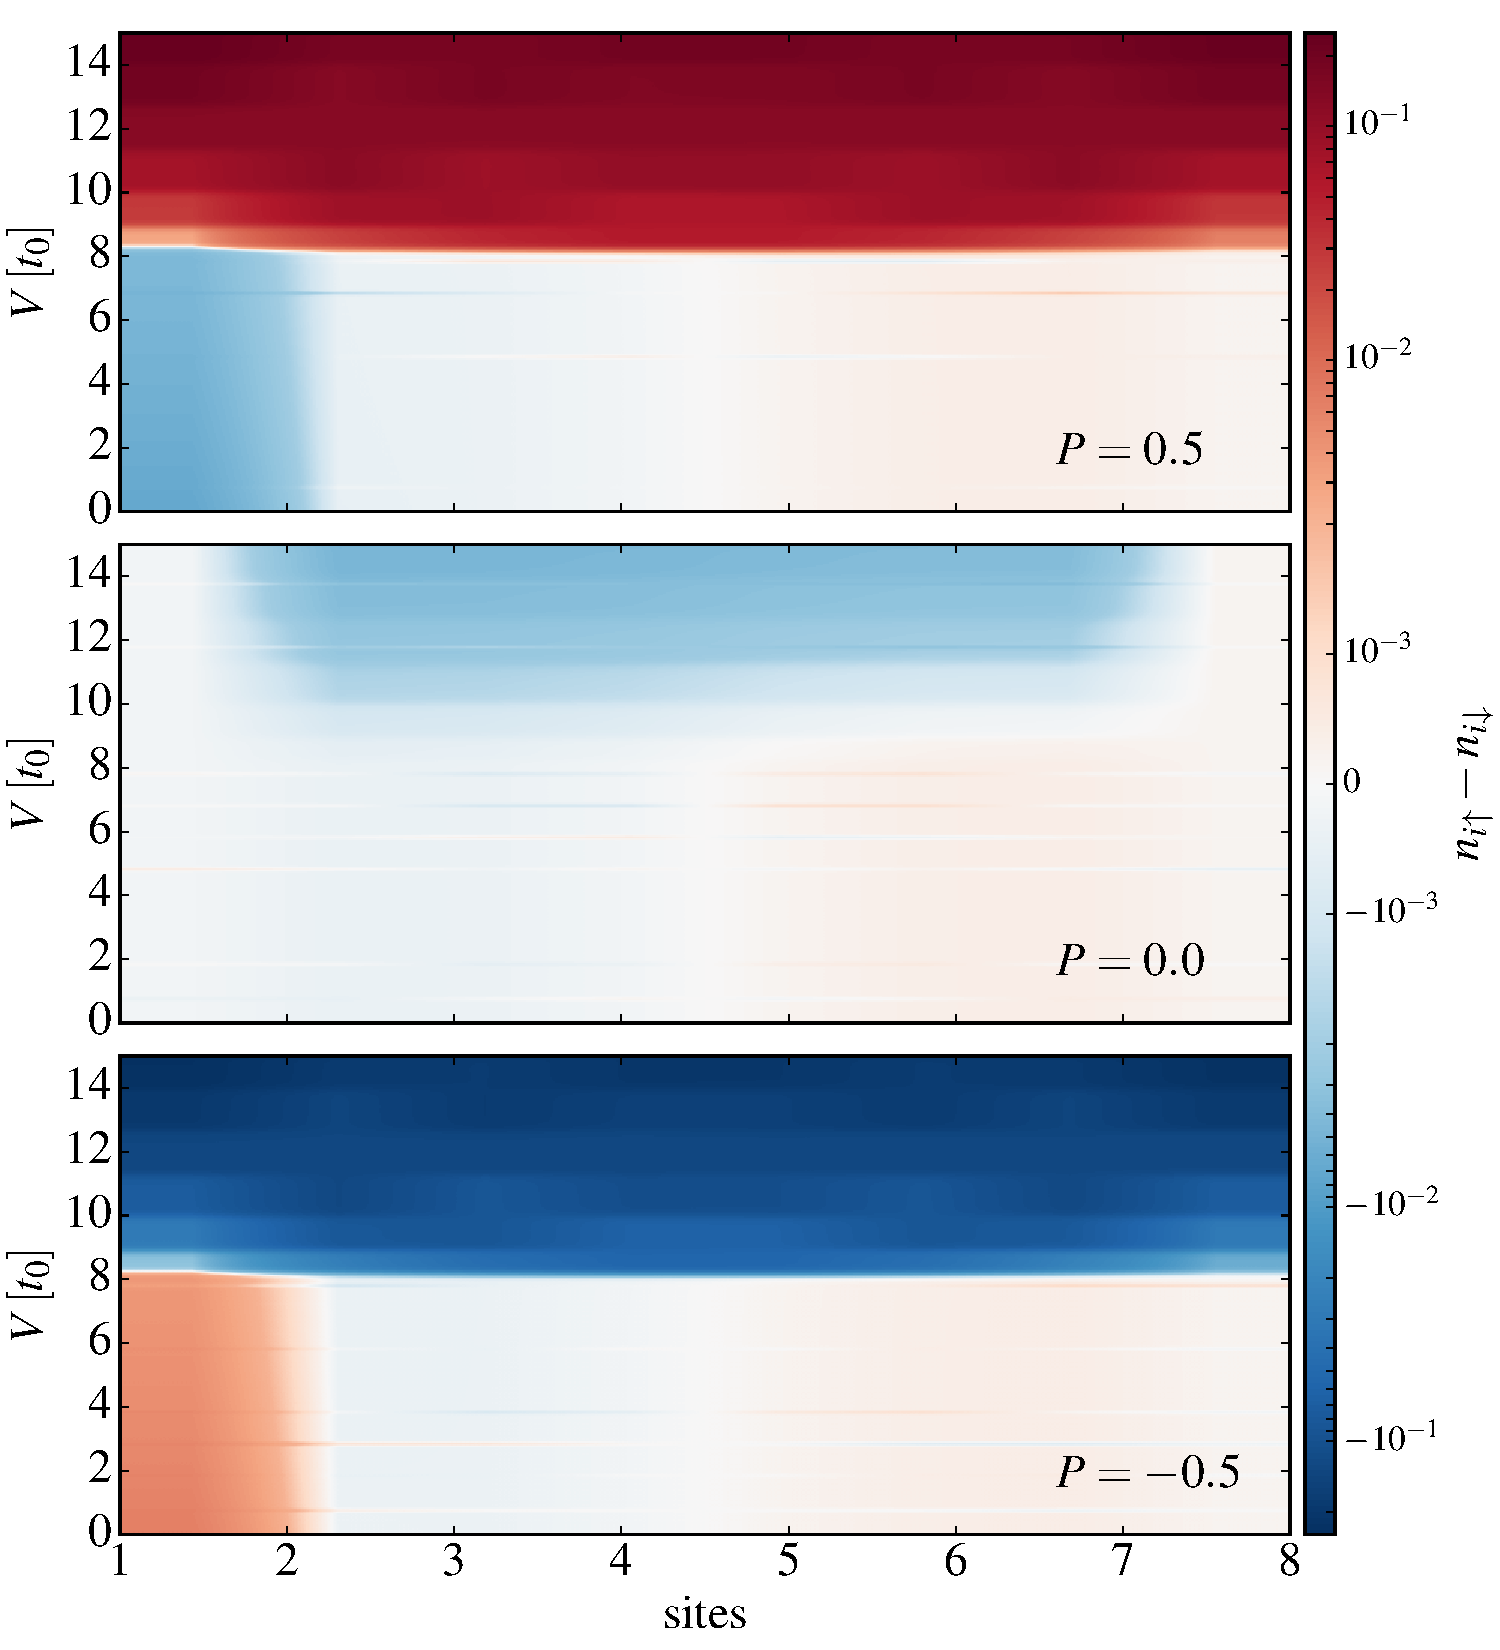
\includegraphics[width=0.8\textwidth]{figs/MF-HEOM_2x4_Sz_steady_PVar.pdf}
	\caption{$\mathbb{M}=2\times 4$}
\end{figure}
Steady state electronic spin polarization in real-space increases (decrases) step-wise with increasing voltage if $P=0.5$ ($P=-0.5$). 
This is explained in the resonant transport model, because the eigenstates of the central Hamiltonian are not localized on single sites, but are extended over the full system. But when a voltage is applied, these eigenstates can be occupied. The voltage at which the steps occur correspond to a resonance condition.

\section{Ehrenfest Dynamics in the Coupled molecule}
\subsection{Test of nuclear dynamics}
Put here a plot of the comparison between analytic and numerical result for the nuclear dynamics for the case of $g=0$.
Put here numerical comparison between quantum Ehrenfest Force calculated by hand and the one obtained in the code.
\subsubsection{Reduction to molecular dynamics for zero electron-phonon coupling}
For vanishing electron-phonon coupling, the nuclear dynamics reduces to a purely molecular dynamics integration. 
Then, the Hamiltonian reduces to 
\begin{equation}
	H = \sum_i \frac{\omega_i}{2}\left(\omega_i X_i^2 + P_i^2\right) + H_\mathrm{el}
\end{equation}
where $H_\mathrm{el}$ is the purely electronic part of the total Hamiltonian.
Since the vibrational modes are not coupled among each other, a single mode is considered.
Then the Hamilton's equation of motion for vibrational coordinates and momenta then read
\begin{align}
	\frac{\dif X}{\dif t} &= \frac{\partial H}{\partial P} = \omega P\\
	\frac{\dif P}{\dif t} &= -\frac{\partial H}{\partial X} = -\omega^2 X\\
	X(0) &= 1, P(0) = 0
\end{align}
the solution of which can be found analytically as
\begin{align}
	X(t) &= \cos(\omega^{3/2}t),\label{eq:AnalyticalVib1}\\
	P(t) &= -\sqrt{\omega} \sin(\omega^{3/2}t).\label{eq:AnalyticalVib2}
\end{align}
The numerical integration agrees with the analytical results, as shown in \cref{fig:Comparison_Vib_Analytical}.
\begin{figure}[!h]
	\centering
	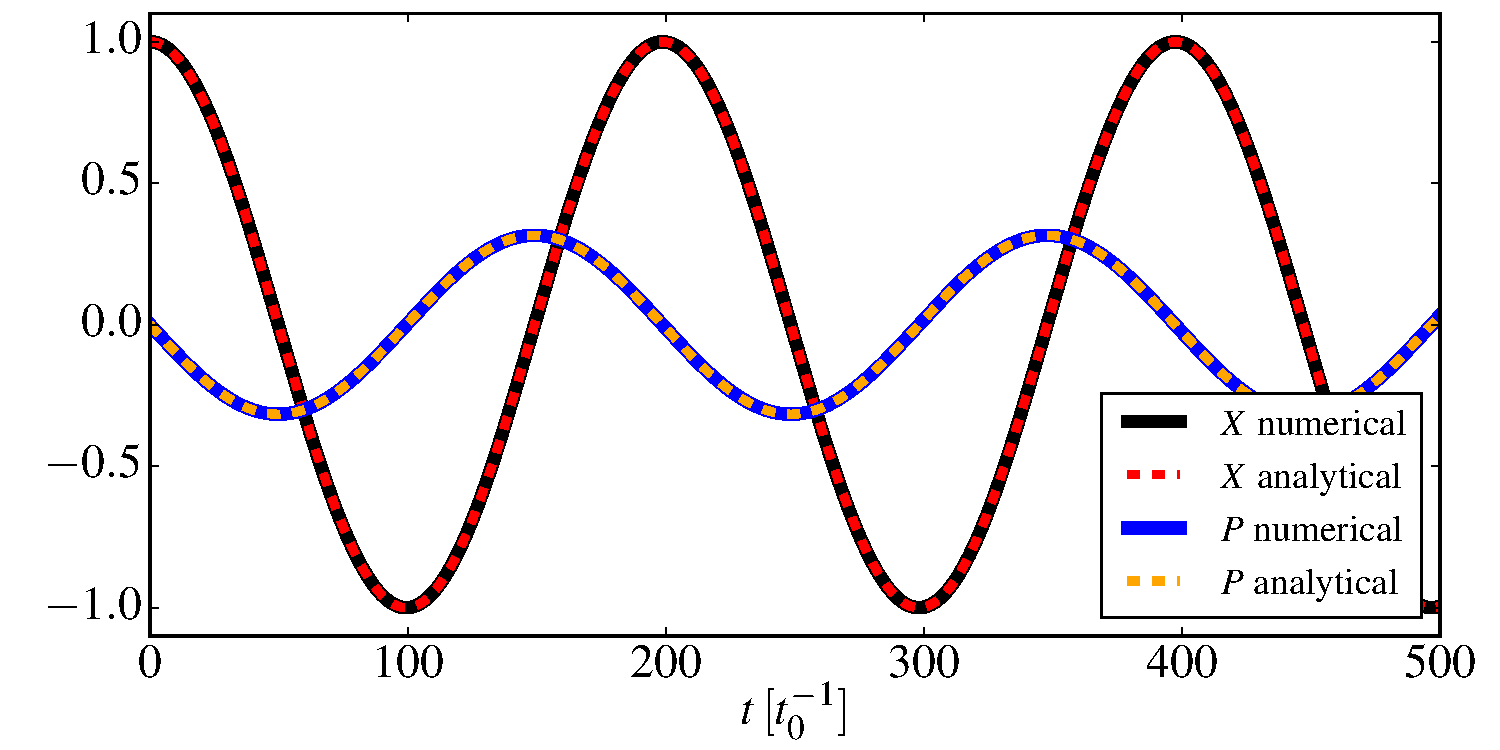
\includegraphics[width=0.7\textwidth]{figs/Decoupled_vibrational_dynamics.pdf}
	\caption{Numerical $X$, $P$ (black, blue line) and analytical functions (\cref{eq:AnalyticalVib1,eq:AnalyticalVib2}, dashed lines) for $\omega = 0.1$.}\label{fig:Comparison_Vib_Analytical}
\end{figure}\\
The dynamics of the electronic system follows time-dependent Schrödinger equation
\begin{align}
	\frac{\dif}{\dif t} \vert\psi(t)\rangle &= -iH \vert\psi(t)\rangle\\
	\vert\psi(0)\rangle &= \begin{pmatrix}
		1\\
		0
	\end{pmatrix}
\end{align}
with the Hamiltonian
\begin{equation}
	H = \begin{pmatrix}
		0 & -t_0\\
		-t_0 & 0
	\end{pmatrix}.
\end{equation}
The solution is 
\begin{equation}
	\vert\psi(t)\rangle = \begin{pmatrix}
		\cos(t_0 t)\\
		i\sin(t_0 t)
	\end{pmatrix}
\end{equation}
\subsubsection{Initial distribution of vibrational phase space coordinates}
As in the usual multi-trajectory Ehrenfest methodology, the initial vibrational phase space coordinates are sampled from the Boltzmann distribution for a harmonic oscillator in its ground state
\begin{equation}
	\rho(\{X\},\{P\}) = \prod_j \frac{\alpha_j}{\pi} \exp\left[-\frac{\alpha_j}{\omega_j} \left(P_j^2+\omega_j^2X_j^2\right)\right],
\end{equation} 
with $\alpha_j = \tanh(\frac{1}{2}\beta \omega_j)$. In the numerical calculation, pseudo-random numbers are sampled from this distribution at the initial time. \Cref{fig:Comparison_Pdist_analytical_numerical} shows a comparison of the analytical probability density distribution with a histogram of numbers randomly sampled from this distribution.
\begin{figure}[!h]
	\centering
	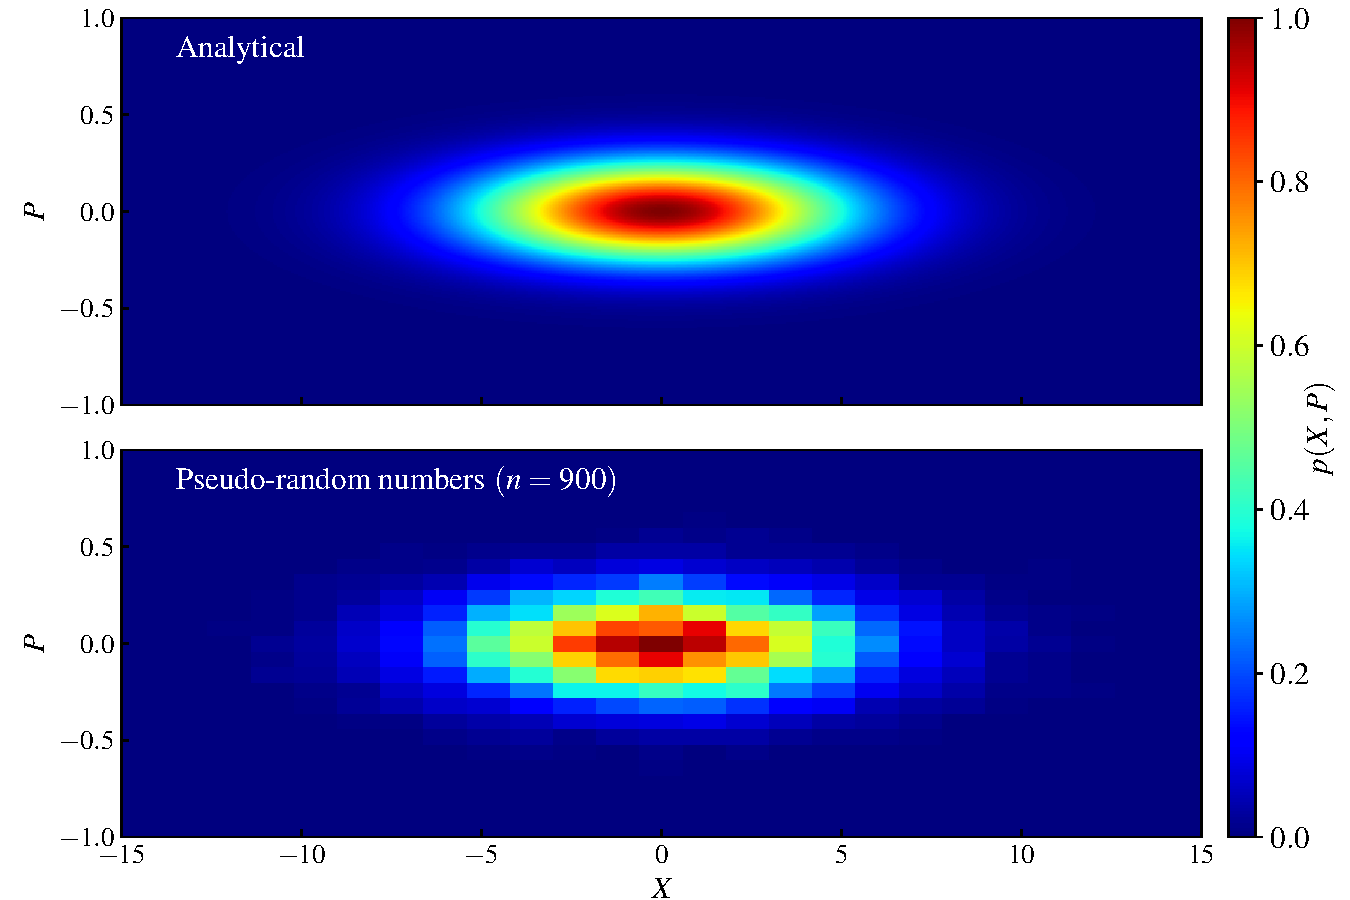
\includegraphics[width=1.0\textwidth]{figs/Comparison_Pdist_analytical_numerical.pdf}
	\caption{Comparison of analytical harmonic oscillator Boltzmann probability density distribution ($\omega = 0.05$, $\beta = 40$) with pseudo-random numbers sampled from the same distribution (samplesize $n=900$).}\label{fig:Comparison_Pdist_analytical_numerical}
\end{figure}
\subsection{Existence of NESS}
Can we make a ``phase diagram'' when a NESS exists? From the data, its easy. Everytime $\mu_L,\mu_R  \gg \varepsilon_n$, or $\mu_L\gg \varepsilon_n$ and $\mu_R \ll \varepsilon_0$, there exists a unique NESS. However, for voltages in the middle of the band, there is no NESS. 
Analytically, I don't know.
In a sense, there is never a NESS in the model I'm investigating. If there is a current, then the current-operator is non-zero. But if the current operator is non-zero, there is coupling between the electrons and the phonons. 
\subsection{Time-dependent Currents}
Show that in the Ehrenfest approach, currents are not reaching a steady state for sufficiently high bias.
Show $(t,V)$ imshow of current.
\subsection{Time-dependent Populations}
Show that populations are also not stationary for long times, but switch depending on the positions of the phonons.
Show $(t,V)$ imshow of population on a single site.
Show $(t,\mathrm{site})$ imshow of all populations on all sites for different times.
Can be explained with spectrum which is now time-dependent under the influence of phonons.
Quantization of vibrational motion. Show FFT of population dynamics. Relation to phonon-frequencies. If matching, then there are quanta of vibration exchanged between electrons and vibrations.
\subsection{Time-dependence of spectrum}
Berry phase effects? 
\subsection{Time-dependent vibrational phase space density}
Show that the phase space density for the nuclear DoF deviates from the initial probability density, and that it still can be well described by a Gaussian/coherent state. Therefore, resampling techniques cannot and should not be applied, because otherwise the deviation of the vibrational phase space density from the initial one is not accounted for correctly.
Explain why currents and populations never reach steady state (because a current is associated with electron hopping, but electron hopping is depending on the positions of the phonons, and hopping induces vibrational dynamics). 
Parameters: $w_0=0.05$, $N_\mathrm{traj} = 900$.
\begin{figure}[!h]
	\centering
	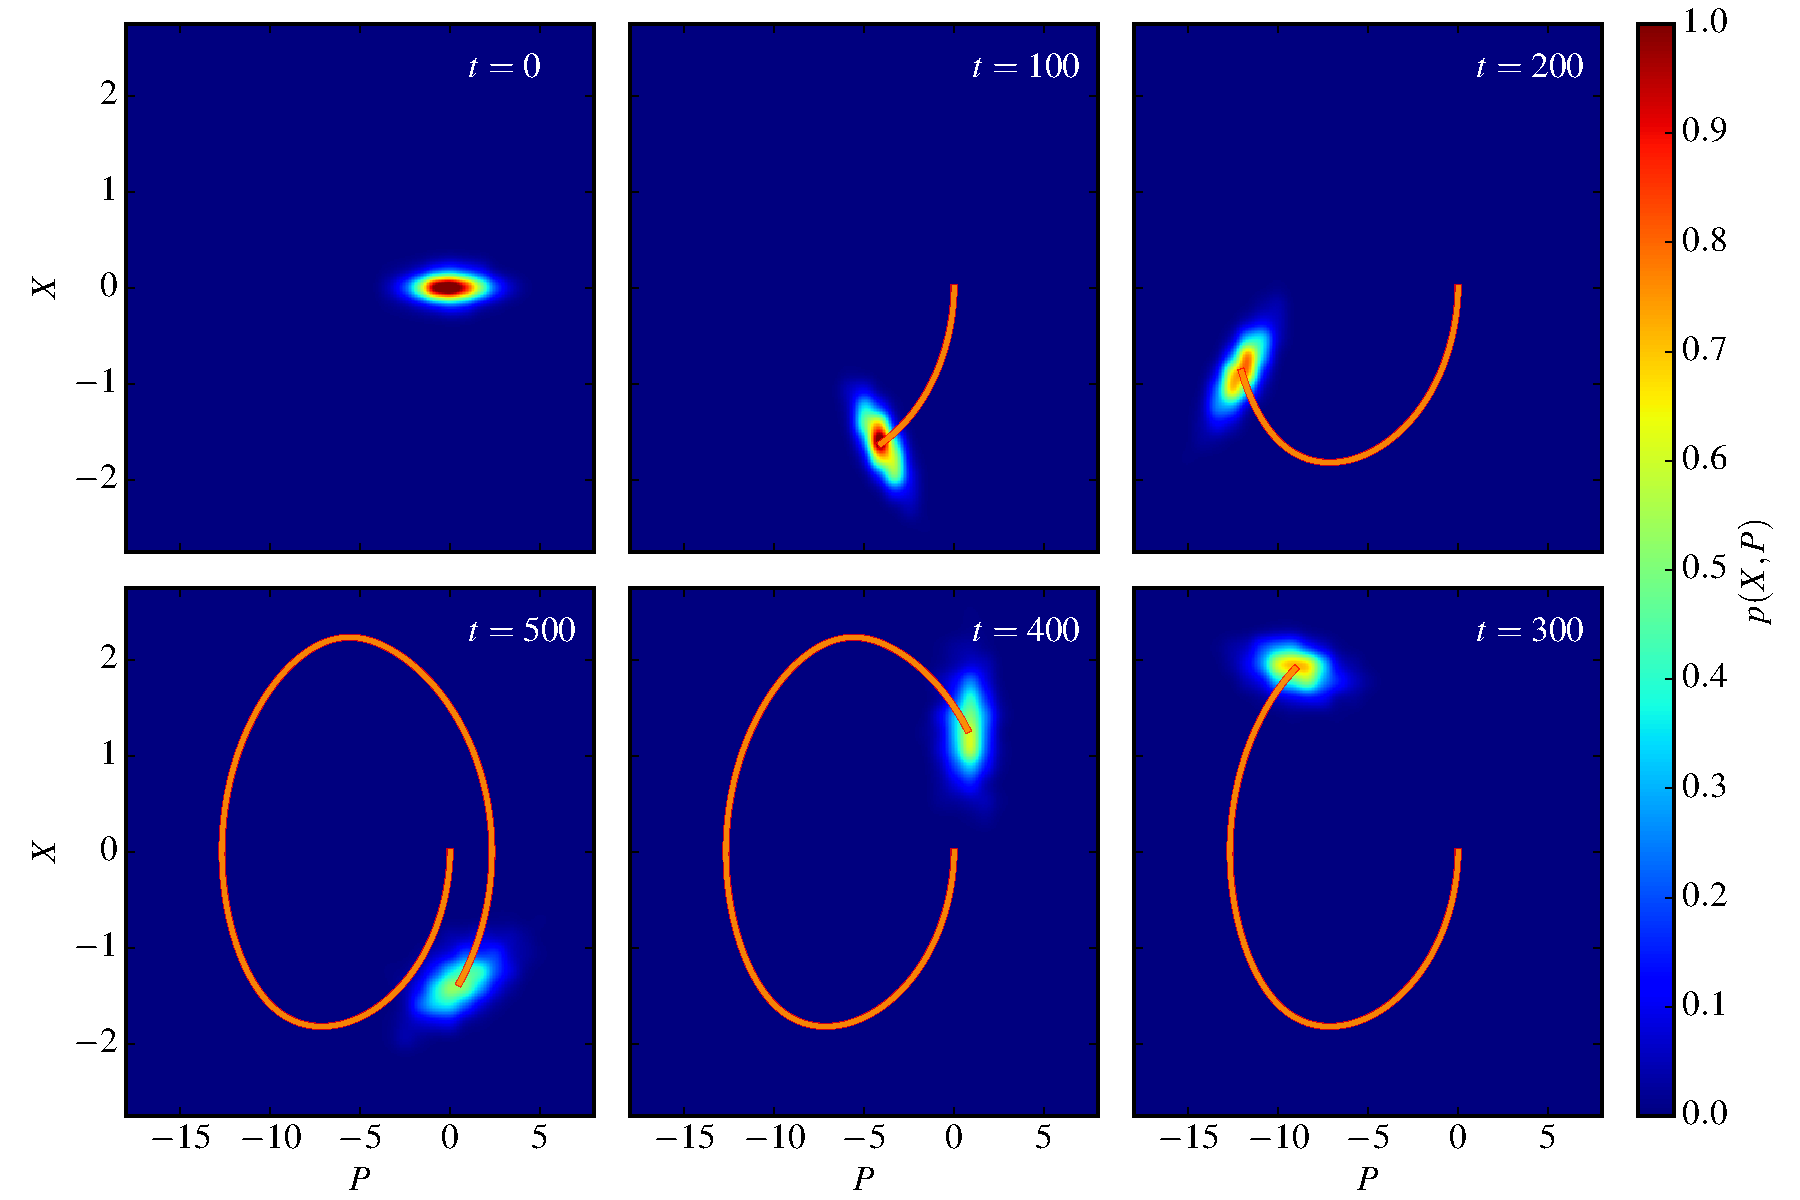
\includegraphics[width=1.0\textwidth]{figs/1x3_PDist_Evo_site0.pdf}
	\caption{Time-evolution of vibrational phase-space probability density at the bond between sites 1 and 2 for $\mathbb{M}=1\times 3$. Parameters are: $t_0 = 1, t_1 = 0.1t_0, \lambda_0 = t_0/40, \lambda_1 = 0.1\lambda_0, \omega_0 = 0.05t_0, P = 0.5$, and $V=10t_0$.}
\end{figure}
Same figure with $P=-0.5,P=0.0$, and $\lambda_1 = 0$ and maybe different voltage.
\subsection{Magnetoresistance}


\printbibliography
\end{document}




